\documentclass{ximera}
\graphicspath{  %% When looking for images,
{./}            %% look here first,
{./pictures/}   %% then look for a pictures folder,
{../pictures/}  %% which may be a directory up.
{../../pictures/}  %% which may be a directory up.
{../../../pictures/}  %% which may be a directory up.
{../../../../pictures/}  %% which may be a directory up.
}

\usepackage{listings}
\usepackage{circuitikz}
\usepackage{xcolor}
\usepackage{amsmath,amsthm}
\usepackage{subcaption}
\usepackage{graphicx}
\usepackage{tikz}
\usepackage{tikz-3dplot}
\usepackage{amsfonts}
\usepackage{mdframed} % For framing content
\usepackage{tikz-cd}

  \renewcommand{\vector}[1]{\left\langle #1\right\rangle}
  \newcommand{\arrowvec}[1]{{\overset{\rightharpoonup}{#1}}}
  \newcommand{\ro}{\texttt{R}}%% row operation
  \newcommand{\dotp}{\bullet}%% dot product
  \renewcommand{\l}{\ell}
  \let\defaultAnswerFormat\answerFormatBoxed
  \usetikzlibrary{calc,bending}
  \tikzset{>=stealth}
  




%make a maroon color
\definecolor{maroon}{RGB}{128,0,0}
%make a dark blue color
\definecolor{darkblue}{RGB}{0,0,139}
%define the color fourier0 to be the maroon color
\definecolor{fourier0}{RGB}{128,0,0}
%define the color fourier1 to be the dark blue color
\definecolor{fourier1}{RGB}{0,0,139}
%define the color fourier 1t to be the light blue color
\definecolor{fourier1t}{RGB}{173,216,230}
%define the color fourier2 to be the dark green color
\definecolor{fourier2}{RGB}{0,100,0}
%define teh color fourier2t to be the light green color
\definecolor{fourier2t}{RGB}{144,238,144}
%define the color fourier3 to be the dark purple color
\definecolor{fourier3}{RGB}{128,0,128}
%define the color fourier3t to be the light purple color
\definecolor{fourier3t}{RGB}{221,160,221}
%define the color fourier0t to be the red color
\definecolor{fourier0t}{RGB}{255,0,0}
%define the color fourier4 to be the orange color
\definecolor{fourier4}{RGB}{255,165,0}
%define the color fourier4t to be the darker orange color
\definecolor{fourier4t}{RGB}{255,215,0}
%define the color fourier5 to be the yellow color
\definecolor{fourier5}{RGB}{255,255,0}
%define the color fourier5t to be the darker yellow color
\definecolor{fourier5t}{RGB}{255,255,100}
%define the color fourier6 to be the green color
\definecolor{fourier6}{RGB}{0,128,0}
%define the color fourier6t to be the darker green color
\definecolor{fourier6t}{RGB}{0,255,0}

%New commands for this doc for errors in copying
\newcommand{\eigenvar}{\lambda}
%\newcommand{\vect}[1]{\mathbf{#1}}
\renewcommand{\th}{^{\text{th}}}
\newcommand{\st}{^{\text{st}}}
\newcommand{\nd}{^{\text{nd}}}
\newcommand{\rd}{^{\text{rd}}}
\newcommand{\paren}[1]{\left(#1\right)}
\newcommand{\abs}[1]{\left|#1\right|}
\newcommand{\R}{\mathbb{R}}
\newcommand{\C}{\mathbb{C}}
\newcommand{\Hilb}{\mathbb{H}}
\newcommand{\qq}[1]{\text{#1}}
\newcommand{\Z}{\mathbb{Z}}
\newcommand{\N}{\mathbb{N}}
\newcommand{\q}[1]{\text{``#1''}}
%\newcommand{\mat}[1]{\begin{bmatrix}#1\end{bmatrix}}
\newcommand{\rref}{\text{reduced row echelon form}}
\newcommand{\ef}{\text{echelon form}}
\newcommand{\ohm}{\Omega}
\newcommand{\volt}{\text{V}}
\newcommand{\amp}{\text{A}}
\newcommand{\Seq}{\textbf{Seq}}
\newcommand{\Poly}{\textbf{P}}
\renewcommand{\quad}{\text{    }}
\newcommand{\roweq}{\simeq}
\newcommand{\rowop}{\simeq}
\newcommand{\rowswap}{\leftrightarrow}
\newcommand{\Mat}{\textbf{M}}
\newcommand{\Func}{\textbf{Func}}
\newcommand{\Hw}{\textbf{Hamming weight}}
\newcommand{\Hd}{\textbf{Hamming distance}}
\newcommand{\rank}{\text{rank}}
\newcommand{\longvect}[1]{\overrightarrow{#1}}
% Define the circled command
\newcommand{\circled}[1]{%
  \tikz[baseline=(char.base)]{
    \node[shape=circle,draw,inner sep=2pt,red,fill=red!20,text=black] (char) {#1};}%
}

% Define custom command \strikeh that just puts red text on the 2nd argument
\newcommand{\strikeh}[2]{\textcolor{red}{#2}}

% Define custom command \strikev that just puts red text on the 2nd argument
\newcommand{\strikev}[2]{\textcolor{red}{#2}}

%more new commands for this doc for errors in copying
\newcommand{\SI}{\text{SI}}
\newcommand{\kg}{\text{kg}}
\newcommand{\m}{\text{m}}
\newcommand{\s}{\text{s}}
\newcommand{\norm}[1]{\left\|#1\right\|}
\newcommand{\col}{\text{col}}
\newcommand{\sspan}{\text{span}}
\newcommand{\proj}{\text{proj}}
\newcommand{\set}[1]{\left\{#1\right\}}
\newcommand{\degC}{^\circ\text{C}}
\newcommand{\centroid}[1]{\overline{#1}}
\newcommand{\dotprod}{\boldsymbol{\cdot}}
%\newcommand{\coord}[1]{\begin{bmatrix}#1\end{bmatrix}}
\newcommand{\iprod}[1]{\langle #1 \rangle}
\newcommand{\adjoint}{^{*}}
\newcommand{\conjugate}[1]{\overline{#1}}
\newcommand{\eigenvarA}{\lambda}
\newcommand{\eigenvarB}{\mu}
\newcommand{\orth}{\perp}
\newcommand{\bigbracket}[1]{\left[#1\right]}
\newcommand{\textiff}{\text{ if and only if }}
\newcommand{\adj}{\text{adj}}
\newcommand{\ijth}{\emph{ij}^\text{th}}
\newcommand{\minor}[2]{M_{#2}}
\newcommand{\cofactor}{\text{C}}
\newcommand{\shift}{\textbf{shift}}
\newcommand{\startmat}[1]{
  \left[\begin{array}{#1}
}
\newcommand{\stopmat}{\end{array}\right]}
%a command to give a name to explorations and hints and theorems
\newcommand{\name}[1]{\begin{centering}\textbf{#1}\end{centering}}
\newcommand{\vect}[1]{\vec{#1}}
\newcommand{\dfn}[1]{\textbf{#1}}
\newcommand{\transpose}{\mathsf{T}}
\newcommand{\mtlb}[2][black]{\texttt{\textcolor{#1}{#2}}}
\newcommand{\RR}{\mathbb{R}} % Real numbers
\newcommand{\id}{\text{id}}

\author{Zack Reed} %PEter Selinger
\title{Matrices and Systems of Equations}
\begin{document}
\begin{abstract}
Here we introduce one of the most prevalent applications of matrices and vectors, the solving of systems of equations.
\end{abstract}
\maketitle



\tikzstyle geometryDiagrams=[ultra thick,color=blue!50!black]

\section{Matrix-Vector Products Yield Systems of Equations}

Systems of linear equations are everywhere, and one of the key applications of vectors and matrices is the efficient solving of such systems. Let's begin with an example from circuits!

\begin{exploration}\name{Circuit Analysis and Systems of Equations}

  The tools of linear algebra can be used to study the application of resistor networks. 

There is a difference in electric potential between the $+$ and $-$ terminals of a battery, measured in volts. This difference in potential causes a current to flow through a circuit. The current is measured in amperes (amount of charge per second) and is slowed by resistors in the circuit. 

An example of an electrical circuit is below.

\begin{center}
  %\scalebox{0.8}{
  %  \begin{circuitikz}[american] \draw
  %    (0,0) to [battery1, v^= $18\volt$~~] (0,4)
  %    (0,0) to [R = $2 \ohm$] (4,0)
  %    to [R = $4 \ohm$] (4,4)
  %    (0,4) to [R =$2 \ohm$] (4,4)
  %    (2,2) node[scale=4]{$\circlearrowleft$}
  %    (2,2) node{$I_1$}
  %    ;
  %  \end{circuitikz}
  %}
  %include image from circuit-1
  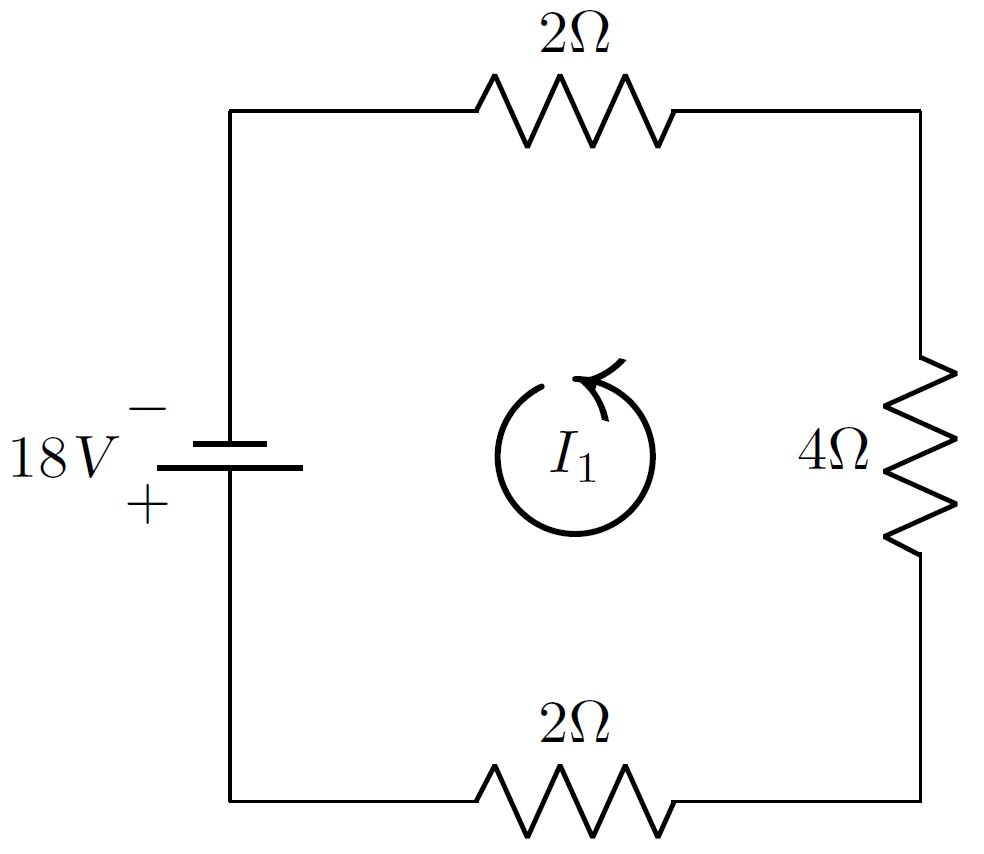
\includegraphics{circuits-1.png}
\end{center}

\noindent
The jagged lines %(\begin{circuitikz}[baseline=-0.5ex] \draw (0,0) to
  %[R] (2,0); \end {circuitikz}) 
  denote resistors and the numbers next
to them give their resistance%
\index{resistance} in ohms (i.e. volts/amperes), written as $\ohm$. The voltage%
\index{voltage} source %(\begin{circuitikz}[baseline=-0.5ex] \draw
  %(0,0) to [/tikz/circuitikz/bipoles/length=0.75cm, battery1]
  %(1,0); \end {circuitikz}) 
  causes the current%
\index{current} to flow in the direction from the longer of the two
lines toward the shorter\footnote{By {\em current}, we always mean the
  {\em conventional current}, which flows from plus to minus. It is
  the opposite of the electron flow, which goes from minus to plus.}.
Voltage is measured in volts, written as $\volt$.  The current for a
circuit is labelled $I_k$, and is measured in amperes, written as
$\amp$.

In the above figure, the current $I_1$ has been labelled with an arrow
in the counterclockwise direction. This is an entirely arbitrary
decision and we could have chosen to label the current in the
counterclockwise direction.  With our choice of direction here, we
define a positive current to flow in the counterclockwise direction
and a negative current to flow in the clockwise direction.

The goal of this section is to use the values of resistors and voltage
sources in a circuit to determine the current. An essential theorem
for this application is Kirchhoff's law%
\index{Kirchhoff's law}.

\begin{theorem}{Kirchhoff's law}{kirchhoff-law}
  The sum of the resistance ($R$) times the amperes ($I$) in the
  counterclockwise direction around a loop equals the sum of the
  voltage sources ($V$) in the same direction around the loop.
\end{theorem}

Kirchhoff's law allows us to set up a system of linear equations and
solve for any unknown variables. When setting up this system, it is
important to trace the circuit in the counterclockwise direction. If a
resistor or voltage source is crossed against this direction, the
related term must be given a negative sign.

We will explore this in the next example where we determine the value
of the current in the initial diagram.

\begin{example}\name{Solving for current}
  Applying Kirchhoff's Law to the diagram below, determine the value for $I_1$.

  \begin{center}
    %\scalebox{0.8}{
    %  \begin{circuitikz}[american,scale=0.8] \draw
    %%    (0,0) to [battery1, v^= $18\volt$~~] (0,4)
     %   (0,0) to [R = $2 \ohm$] (4,0)
     %   to [R = $4 \ohm$] (4,4)
     %   (0,4) to [R =$2 \ohm$] (4,4)
     %   (2,2) node[scale=4]{$\circlearrowleft$}
     %   (2,2) node{$I_1$}
     %   ;
     % \end{circuitikz}
    %}
    %include image from circuit-2
    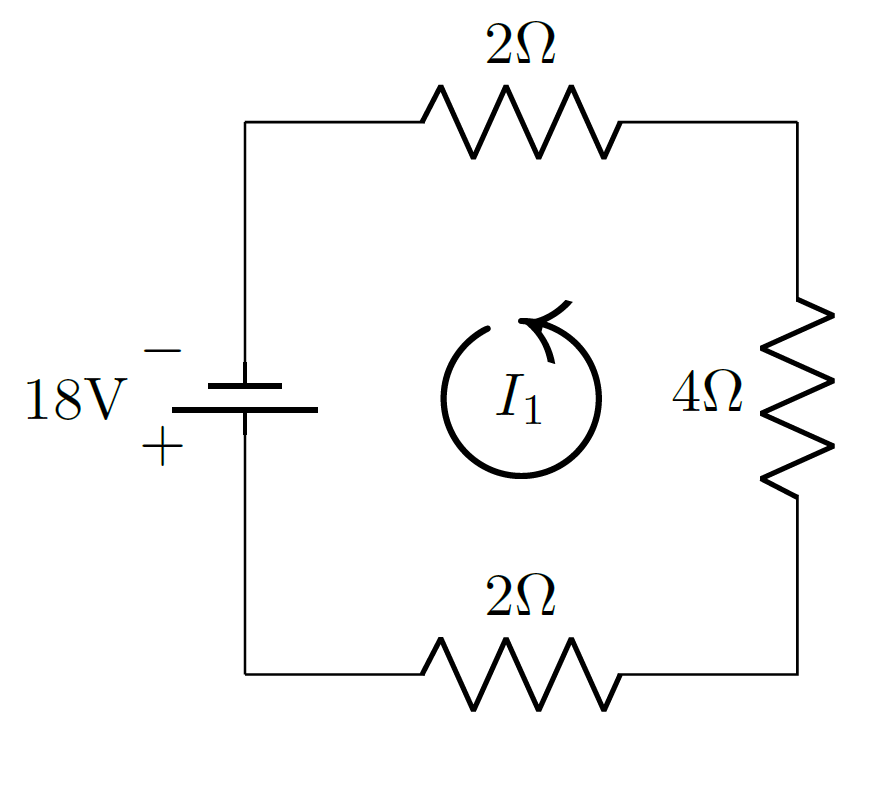
\includegraphics{circuits-2.png}
  \end{center}



\begin{solution}
  Begin in the bottom left corner, and trace the circuit in the
  counterclockwise direction. At the first resistor, multiplying
  resistance and current gives $2I_1$. Continuing in this way through
  all three resistors gives $2I_1 + 4I_1 + 2 I_1$. This must equal the
  voltage source in the same direction. Notice that the direction of
  the voltage source matches the counterclockwise direction specified,
  so the voltage is positive.

  Therefore the equation is given by
  \begin{eqnarray*}
    2I_1 + 4I_1 + 2 I_1 &=& 18, \\
  \end{eqnarray*}

  Our unknown current is $I_1$, and we can solve for $I_1$ in the usual algebraic way. The equation simplifies to

  and the solution is
  \begin{eqnarray*}
    8I_1 &=& 18, \\
    I_1 &=& \answer{9/4} \amp.
  \end{eqnarray*}
  Remember that the unit for current is $\amp$. Since the answer is positive, this confirms that the current flows
  counterclockwise.
\end{solution}

\end{example}

\begin{example}\name{Unknown currents}
  The diagram below consists of four circuits. The current ($I_k$) in
  the four circuits is denoted by $I_1$, $I_2$, $I_3$, $I_4$. Using
  Kirchhoff's Law, write an equation for each circuit and solve for
  each current.

  \begin{center}
    %\scalebox{0.8}{
    %  \begin{circuitikz}[american, scale=0.7] \draw
    %    (0,0) to [battery1, v^= $18\volt$~~] (0,4)
    %    (0,0) to [R = $2 \ohm$] (4,0)
    %    to [R = $4 \ohm$] (4,4)
    %    (0,4) to [R =$2 \ohm$] (4,4)
    %    (6,4) to [battery1, v_= \raisebox{1ex}{$27\volt$}] (4,4)
    %    (6,4) to [R = $3 \ohm$] (8,4)
    %    to [R = $1 \ohm$] (8,0)
    %    (4,0) to [R = $6 \ohm$] (8,0)
    %    to [R = $2 \ohm$] (8,-4)
    %    to [R = $3 \ohm$] (4,-4)
    %    to [R = $1 \ohm$] (4,0)
    %    (4,-4)to [R = $5 \ohm$] (0,-4)
    %    (0,0) to [battery1, v_= $23\volt$~~] (0,-4)
    %    (2,2) node[scale=3]{$\circlearrowleft$}
    %    (2,2) node{$I_2$}
    %    (6,2) node[scale=3]{$\circlearrowleft$}
    %    (6,2) node{$I_3$}
    %    (6,-2) node[scale=3]{$\circlearrowleft$}
    %    (6,-2) node{$I_4$}
    %    (2,-2) node[scale=3]{$\circlearrowleft$}
    %    (2,-2) node{$I_1$}
    %    ;
    %  \end{circuitikz}
    %}
    %include image from circuit-3
    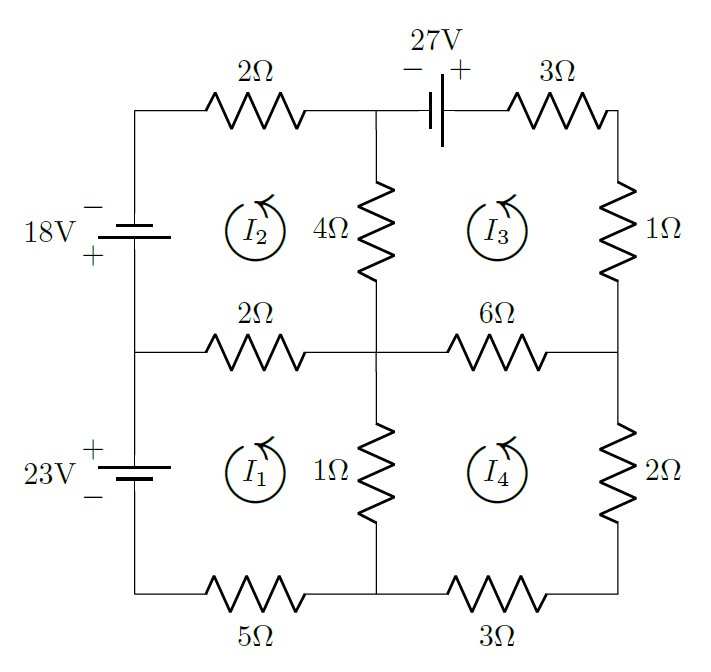
\includegraphics{circuits-3.png}
  \end{center}

  Starting with the top left circuit, multiply the resistance by the
  current and sum the resulting products. Specifically, consider the
  resistor labelled $2 \ohm$ that is part of the circuits of $I_1$ and
  $I_2$. 
  
  Notice that current $I_2$ runs through this in a positive
  (counterclockwise) direction, and $I_1$ runs through in the opposite
  (negative) direction. The product of resistance and current is then
  $2 (I_2 - I_1) = 2I_2 - 2I_1$.  
  
  Continue in this way for each
  resistor, and set the sum of the products equal to the voltage
  source to write the equation:
  \begin{equation*}
    2I_2-2I_1+4I_2-4I_3+2I_2=18.
  \end{equation*}
  The above process is used on each of the other three circuits, and
  the resulting equations are:

  \noindent
  Upper right circuit:
  \begin{equation*}
    4I_3 - 4I_2 + 6I_3 - 6I_4 + I_3 + 3I_3 = -27.
  \end{equation*}
  Lower right circuit:
  \begin{equation*}
    3I_4 + 2I_4 + 6I_4 - 6I_3 + I_4 - I_1 = 0.
  \end{equation*}
  Lower left circuit:
  \begin{equation*}
    5I_1+I_1-I_4+2I_1-2I_2=-23.
  \end{equation*}

  Notice that the voltage for the upper right and lower left circuits
  are negative due to the clockwise direction they indicate. The
  resulting system has four equations in four variables. 

  \begin{remark}

    This first example of a system of equations highlights some important assumptions that we'll make in order to utilize the tools from linear algebra.

    First, the system is complex because each equation must be satisfied simultaneously for the entire system to have a solution. We saw this briefly when examining the span of vector sets, that any solution must satisfy all equations in the system.

    Second, for the purpose of this course we're only going to consider \emph{linear} systems. In true fashion, we mean that all elements of the system must be the results of addition or scalar multiplication. This is a little different from the vector example, as technically the variables are scalars, but what we mean here is that you can only construc the system by multiplying scalars to variables, or by adding products together. 

    This brings the following definitions.

    \begin{definition}\name{Linear equation}
      A \textbf{linear equation}%
      \index{linear equation} is an equation of the form
      \begin{equation*}
        a_1x_1 + a_2x_2 + \ldots + a_nx_n = b.
      \end{equation*}
      Here, $a_1,\ldots,a_n$ are real numbers called the
      \textbf{coefficients}%
      \index{coefficient} of the equation, $b$ is a real number called the
      \textbf{constant term}%
      \index{constant term} of the equation, and $x_1,\ldots,x_n$ are
      \textbf{variables}%
      \index{variable}.
    \end{definition}

    \begin{example}{Linear vs. non-linear equation}{linear-vs-non-linear}
      Which of the following equations are linear?
      \begin{equation*}
        \begin{array}{cc}
          2x+3y=5 & is \wordChoice{\choice[correct]{linear},\choice{non linear}}\\
          2x^2+3y=5 & is \wordChoice{\choice{linear},\choice[correct]{non linear}}\\
          2\sqrt{x} + 3y = 5 & is \wordChoice{\choice{linear},\choice[correct]{non linear}}\\
          (\sqrt{2}) x + 3y = 5^2 & is \wordChoice{\choice[correct]{linear},\choice{non linear}}
        \end{array}
      \end{equation*}
    \end{example}

    We then need to define a system of linear equations.

    \begin{definition}\name{System of linear equations}
      A \textbf{system of linear equations}%
      \index{system of linear equations} is a list of equations
      \begin{equation*}
        \begin{array}{c@{~}c@{~}c}
          a_{11}x_1+a_{12}x_2+\ldots+a_{1n}x_n&=&b_1 \\
          a_{21}x_1+a_{22}x_2+\ldots+a_{2n}x_n&=&b_2 \\
          \vdots \\
          a_{m1}x_1+a_{m2}x_2+\ldots+a_{mn}x_n&=&b_m,
        \end{array}
      \end{equation*}
      where $a_{ij}$ and $b_i$ are scalars (i.e., real numbers). The above
      is a system of $m$ equations in the $n$ variables
      $x_1,x_2\ldots,x_n$.  As before, the numbers $a_{ij}$ are called the
      \textbf{coefficients}%
      \index{coefficient} and the numbers $b_i$ are called the
      \textbf{constant terms}%
      \index{constant term} of the system of equations.
    \end{definition}

    Finally, we want some terminology for whether at least one solution to a system exists.

    \begin{definition}\name{Consistent and inconsistent systems}
      A system of linear equations is called \textbf{consistent}%
      \index{consistent system}%
      \index{system of linear equations!consistent} if there exists at
      least one solution. It is called \textbf{inconsistent}%
      \index{inconsistent system}%
      \index{system of linear equations!inconsistent} if there is no
      solution.
    \end{definition}

  \end{remark}

\begin{solution}
  
  Let's now return to our linear system of equations and determine whether the system is consistent or inconsistent.

  First, rearranging and simplifying so that we list the variables in order, we have:
  \begin{equation*}
    \begin{array}{r@{~}c@{~}l}
      -2I_1+8I_2-4I_3&=&18, \\
      - 4I_2 + 14I_3 - 6I_4 &=& -27, \\
      -I_1 - 6I_3 + 12I_4 &=& 0, \\
      8I_1-2I_2 - I_4 &=& -23.
    \end{array}
  \end{equation*}

  We're going to solve the system systematically, by rearranging terms and manipulating equations so that we don't alter the solutions at all, but so that we can solve for one variable at a time. This is the same process we use when we solve simple algebraic equations, but we're going to be a little more systematic about it.

  \begin{remark}

  We first need to give ourselves some ways to manipulate the system without changing the solutions. These are called \emph{elementary row operations} (or more typically just elementary operations). The somewhat evocative use of the term \emph{row} should perk our ears to suggest that there will be an explicit connection to matrices down the road!

  \begin{definition}\name{Elementary operations}
    \textbf{Elementary operations}%
    \index{elementary operation} are the
    following operations:
  
    \begin{enumerate}
    \item Interchange the order in which the equations are listed.
  
    \item Multiply any equation by a non-zero scalar.
  
    \item Add a multiple of one equation to another equation.
    \end{enumerate}
  \end{definition}

  \end{remark}

  Let's use these elementary row operations to solve the system. Our goal is to get the system into a form where each equation only has one variable on the left, and one constant on the right. If we can make the system look like this, we'll have found our solution.

  One by one, we'll give each variable a coefficient of $1$, and then eliminate all instances of that variable from the other equations. 
  
  We'll start with $I_1$, let's multiply the first equation by $-1/2$, and then also note any terms with $0$ coefficients so that we keep track of variables more easily. We'll also write the altered equation in red so that we can keep track of our progress.

  \begin{equation*}
    \begin{array}{r@{~}c@{~}l}
      \color{red}I_1-4I_2+2I_3+0I_4&=&\color{red}-9, \\
      0I_1- 4I_2 + 14I_3 - 6I_4 &=& -27, \\
      -I_1 +0I_2 - 6I_3 + 12I_4 &=& 0, \\
      8I_1-2I_2 +0I_3 - I_4 &=& -23.
    \end{array}
  \end{equation*}

  Now, we add a multiple of the first equation to all of the other equations to eliminate $I_1$ from them. Since equation 3 has a coefficient of $-1$ for $I_1$, we'll just add the first equation to the third equation. 

  Since the fourth equation has a coefficient of $8$ for $I_1$, we'll add $-8$ times the first equation to the fourth equation.

  This gives the following system:

  \begin{equation*}
    \begin{array}{r@{~}c@{~}l}
      I_1-4I_2+2I_3+0I_4&=&-9, \\
      0I_1- 4I_2 + 14I_3 - 6I_4 &=& -27, \\
      \color{red}0I_1 - 4I_2 - 4I_3 + 12I_4 &=& \color{red}-9, \\
      \color{red}0I_1+30I_2 - 16I_3 - I_4 &=& \color{red}49.
    \end{array}
  \end{equation*}

  Here's the great part about this process: now that the last three equations have $0I1$, adding a multiple of these equations back to $I_1$ won't change the $I_1$ term, so we've now isolated $I_1$!

  Let's move to $I_2$. We'll multiply the second equation by $-1/4$ so that it has a coefficient of $1$ for $I_2$.

  \begin{equation*}
    \begin{array}{r@{~}c@{~}l}
      I_1-4I_2+2I_3+0I_4&=&-9, \\
      \color{red}0I_1+I_2 - 7/2I_3 + 3/2I_4 &=& \color{red}27/4, \\
      0I_1 - 4I_2 - 4I_3 + 12I_4 &=& -9, \\
      0I_1+30I_2 - 16I_3 - I_4 &=& 49.
    \end{array}
  \end{equation*}

  Now we eliminate $I_2$ from the remaining equations. Let's take some shorthand now to reference the row operations we're doing. We're going to change the first row by adding $4$ times the second row to it, let's denote that by $R_1 \rightarrow R_1 + 4R_2$. We then similarly alter the third and fourth rows, so we denote that by $R_3 \rightarrow R_3 + 4R_2$ and $R_4 \rightarrow R_4 - 30R_2$.

  This yields the system:

  \begin{equation*}
    \begin{array}{r@{~}c@{~}l}
      \color{red}I_1+0I_2-12I_3+6I_4&=&\color{red}18, \\
      0I_1+I_2 - 7/2I_3 + 3/2I_4 &=& 27/4, \\
      \color{red}0I_1 + 0I_2 - 18I_3 + 18I_4 &=& \color{red}18, \\
      \color{red}0I_1+0I_2 + 89I_3 - 46I_4 &=& \color{red}-307/2.
    \end{array}
  \end{equation*}

  Row $3$ is now not too bad, and we can just divide by $-18$ to get $I_3$ by itself. If we do that, and then perform the operations $R_1 \rightarrow R_1 + 12R_3$, $R_2 \rightarrow R_2 + 7/2R_3$, and $R_4 \rightarrow R_4 - 89R_3$, we get:

  \begin{equation*}
    \begin{array}{r@{~}c@{~}l}
      \color{red}I_1+0I_2+0I_3+-6I_4&=&\color{red}6, \\
      \color{red}0I_1+I_2 + 0I_3 -2I_4 &=& \color{red}13/4, \\
      \color{red}0I_1 + 0I_2 + I_3 - I_4 &=& \color{red}-1, \\
      \color{red}0I_1+0I_2 + 0I_3 + 43I_4 &=& \color{red}-129/2.
    \end{array}
  \end{equation*}

  We've found our first variable! If we divide $-129/2$ by $43$, we get $-3/2$, so $I_4 = -3/2$.

  We do need to finish out the system, so we'll do one final round by adding in multiples of $R_4$ to the other rows, doing the following operations: $R_4\rightarrow 1/43 R_4$, $R_1 \rightarrow R_1 + 6R_4$, $R_2 \rightarrow R_2 + 2R_4$, and $R_3 \rightarrow R_3 + R_4$.

  This yeilds the following system: 

  \begin{equation*}
    \begin{array}{r@{~}c@{~}l}
      \color{red}I_1+0I_2+0I_3+0I_4&=&\color{red}-3, \\
      \color{red}0I_1+I_2 + 0I_3 +0I_4 &=& \color{red}1/4, \\
      \color{red}0I_1 + 0I_2 + I_3 + 0I_4 &=& \color{red}-5/2, \\
      \color{red}0I_1+0I_2 + 0I_3 + I_4 &=& \color{red}-3/2.
    \end{array}
  \end{equation*}


  Therefore, the solution to this system of equations is
  \begin{eqnarray*}
    I_1 &=& -3 \amp, \\
    I_2 &=& \frac{1}{4} \amp, \\
    I_3 &=& -\frac{5}{2} \amp, \\
    I_4 &=& -\frac{3}{2} \amp.
  \end{eqnarray*}
  This tells us that currents $I_1, I_3$, and $I_4$ travel clockwise
  while $I_2$ travels counterclockwise.
\end{solution}

Let's recap. We:

\begin{enumerate}

\item solved for the unknown currents in the 4-circuit system by first stating the system of linear equations that describe the balancing of the currents, 
\item systematically altered the system by scaling the rows or adding multiples of one row to another row, 
\item isolated each variable by eliminating it from the other equations.

\end{enumerate}

This method is called \emph{Gaussian elimination}, and underlies an efficient and systematic way that we solve for systems of equations, and (as we'll see next) determine various properties about matrices. 

\begin{remark}

  Remember that vectors are equal only when their corresponding components are equal? We can use that fact here to draw an inherent link between systems of equations and matrices.

  Let's look back at our original system, but again re-state it so that we see which variables have $0$ coefficients.

  \begin{equation*}
    \begin{array}{r@{~}c@{~}l}
      -2I_1+8I_2-4I_3+0I_4&=&18, \\
      0I_1- 4I_2 + 14I_3 - 6I_4 &=& -27, \\
      -I_1 +0I_2- 6I_3 + 12I_4 &=& 0, \\
      8I_1-2I_2 +0I_3- I_4 &=& -23.
    \end{array}
  \end{equation*}

  Stated loosly, we've arranged the system into rows and columns, were the columns are the coefficients of the variables, and the rows are the equations. This is a matrix!

  More importantly, the system lays out exactly the calculations one would make in a matrix-vector product. If we break up the system into columns as if they were column vectors, and factor out the variables, we get:

$$I_1\begin{bmatrix}-2 \\ 0\\-1\\8\end{bmatrix}
+I_2\begin{bmatrix}8 \\ -4\\0\\-2\end{bmatrix}
+I_3\begin{bmatrix}-4 \\ 14\\-6\\0\end{bmatrix}
+I_4\begin{bmatrix}0 \\ -6\\12\\-1\end{bmatrix}
=
\begin{bmatrix}18 \\ -27\\0\\-23\end{bmatrix}$$

This is exactly the calculation you would carry out for the matrix product $C\vec{x}$, where $C$ is the matrix of coefficients in the system and $\vec{x}$ is the vector of unknowns!

Moreover, the constants on the right-sides of the equations can similarly form a vector, $\vec{b}$. 

So any system of equations can be written as a matrix equation

$$A\vec{x} = \vec{b}$$

and solving the system amounts to finding the unknown vector $\vec{x}$ that satisfies the equation.

If we were to state the solution to the system in this way, we would say that the vector

$$\vec{x} = \begin{bmatrix}-3 \\ 1/4\\-5/2\\-3/2\end{bmatrix}$$

satisfies the vector equation 

$$\begin{bmatrix}-2 & 8 & -4 & 0 \\ 0 & -4 & 14 & -6 \\ -1 & 0 & -6 & 12 \\ 8 & -2 & 0 & -1\end{bmatrix}\vec{x} = \begin{bmatrix}18 \\ -27\\0\\-23\end{bmatrix}.$$


\end{remark}

\end{example}

\end{exploration}

\begin{exploration}\name{Chemical Reactions and Matrix Multiplications}

  Let's take a look at another application of systems of equations (now seen as vector equations): balancing chemical reactions.

 Consider
  the chemical reaction%

  \index{chemical reactions!balancing}
  \begin{equation*}
    SnO_2+H_2\rightarrow Sn+H_2O.
  \end{equation*}

Chemical reactions occur when substances (reactants) are transformed to form new substances (products). This happens because the atoms in the reactants are rearranged and new bonds form the products. 

Here the elements involved are tin ($Sn$), oxygen ($O$), and hydrogen
($H$). A chemical reaction occurs that transforms a combination of tin
dioxide ($SnO_2$, one tin and two oxygen) and hydrogen ($H_2$, two hydrogen) into a combination of tin
($Sn$) and water ($H_2O$, two hydrogen one oxygen). 

When considering chemical reactions, we
want to investigate how much of each substance we began with and how
much of each substance is involved in the result.

An important theory we will use here is the {\bf mass balance theory}. It
tells us that we cannot create or delete elements within a chemical
reaction. For example, in the above expression, we must have the same
number of atoms of oxygen, tin, and hydrogen on both sides of the
reaction so that no mass is produced nor descrotyed in the reaction. 

Notice that this is not currently the case.  For example,
there are two oxygen atoms on the left and only one on the right. In
order to fix this, we want to find numbers $x,y,z,w$ such that
\begin{equation*}
  x\;SnO_2+y\;H_2\rightarrow z\;Sn+w\;H_2O,
\end{equation*}
where both sides of the reaction have the same number of atoms of the
various elements.

\begin{example}\name{Balancing the tin, oxygen, hydrogen reaction}

This is a familiar example. We can solve it by setting up a system of
equations in the variables $x,y,z,w$. 

Noting how many atoms are present in each side and part of the reaction, we need
\begin{equation*}
  \begin{array}{cl}
    Sn: & x=z \\
    O: & 2x=w \\
    H: & 2y=2w.
  \end{array}
\end{equation*}

We can rewrite these equations as
\begin{equation*}
  \begin{array}{cl}
    Sn: & x - z = 0 \\
    O: & 2x - w = 0 \\
    H: & 2y - 2w = 0.
  \end{array}
\end{equation*}

Let's think about this example in terms of matrix equations, becuase we can actually do the exact same elementary row operations as in the previous example, but by way of matrix mulitplication, which will save us some time (and lends itself to an intuitive interpretation at the end)

Stating this system in matrix form, we have

\begin{equation*}
  \begin{bmatrix}
    1 & 0 & -1 & 0 \\
    2 & 0 & 0 & -1 \\
    0 & 2 & 0 & -2
  \end{bmatrix}
  \begin{bmatrix}
    x \\
    y \\
    z \\
    w
  \end{bmatrix}
  =
  \begin{bmatrix}
    0 \\
    0 \\
    0
  \end{bmatrix}.
\end{equation*}

So we have a $3\times 4$ matrix $A$ and a $4\times 1$ vector $\vec{x}$ that satisfy the equation $A\vec{x} = \vec{0}$.

\begin{remark}\name{Elementary Matrices}

  We're now going to use matrices to perform the same elementary row operations from the previous example. Remember that we solved the system by 1) replacing one row with another, 2) scaling one row, and 3) adding a multiple of one row to another.

  As it turns out, we can use matrix multiplcation to use perform these same manipulations to matrices. We will call these matrices \emph{elementary matrices}.

  \begin{definition}\name{Row Swapping Matrix}
    The \textbf{row swapping matrix} $E_{ij}$ is the matrix that results from swapping rows $i$ and $j$ of the identity matrix.

    It is the identity matrix with rows $i$ and $j$ swapped.

    For instance, $E_{12}$ performed on a $3\times 3$ matrix would be the matrix

    \begin{equation*}
      \begin{bmatrix}
        0 & 1 & 0 \\
        1 & 0 & 0 \\
        0 & 0 & 1
      \end{bmatrix}
    \end{equation*}

    Notice that the first and second rows are swapped.
  \end{definition}

  \begin{definition}\name{Scaling Matrix}
    The \textbf{scaling matrix} $E_{i}(c)$ is the matrix that results from multiplying row $i$ of the identity matrix by the scalar $c$.

    For instance, $E_{2}(3)$ performed on a $3\times 3$ matrix would be the matrix

    \begin{equation*}
      \begin{bmatrix}
        1 & 0 & 0 \\
        0 & 3 & 0 \\
        0 & 0 & 1
      \end{bmatrix}.
    \end{equation*}

    Notice that the second row is scaled by $3$.
  \end{definition}

  \begin{definition}\name{Row Addition Matrix}
    The \textbf{row addition matrix} $E_{ij}(c)$ is the matrix that results from adding $c$ times row $i$ to row $j$ of the identity matrix.

    For instance, $E_{3,2}(2)$ performed on a $3\times 3$ matrix would be the matrix

    \begin{equation*}
      \begin{bmatrix}
        1 & 0 & 0 \\
        0 & 1 & 0 \\
        0 & 2 & 1
      \end{bmatrix}.
    \end{equation*}

    This will add $2$ times the second row to the third row.
  \end{definition}

\end{remark}

Now let's use these elementary matrices to solve the system of equations.

Our chemical reaction matrix is 

\begin{equation*}
  A = \begin{bmatrix}
    1 & 0 & -1 & 0 \\
    2 & 0 & 0 & -1 \\
    0 & 2 & 0 & -2
  \end{bmatrix}.
\end{equation*}

We want to, as before, isolate each variable by eliminating it from the other equations. This amounts to having a $1$ in each column, and the rest of the column being $0$.

This is already not too difficult for the first two columns of $A$. If we subtract twice the first row from the second row, and then halve the third row, we will have completed this task for the first two columns.

Subtracting twice the first row from the second row is achieved by the {\bf row addition matrix} 

$$E_{2,1}(-2)=\begin{bmatrix}1 & 0 & 0 \\ -2 & 1 & 0 \\ 0 & 0 & 1\end{bmatrix},$$

and halving the third row is achieved by the {\bf scaling matrix}

$$E_{3}(1/2)=\begin{bmatrix}1 & 0 & 0 \\ 0 & 1 & 0 \\ 0 & 0 & .5\end{bmatrix}.$$

We can do this all at once by the matrix multiplciation $E_{3}(1/2)\cdot E_{2,1}(-2)\cdot A$.

We'll confirm this in MATLAB in a moment, but the product is given by 

\begin{equation*}
 \begin{bmatrix}
    1 & 0 & 0 \\
    0 & 1 & 0 \\
    0 & 0 & .5
  \end{bmatrix} \begin{bmatrix}
    1 & 0 & 0 \\
    -2 & 1 & 0 \\
    0 & 0 & 1
  \end{bmatrix} \begin{bmatrix}
    1 & 0 & -1 & 0 \\
    2 & 0 & 0 & -1 \\
    0 & 2 & 0 & -2
  \end{bmatrix} = \begin{bmatrix}
    1 & 0 & -1 & 0 \\
    0 & 0 & 2 & -1 \\
    0 & 1 & 0 & -1
  \end{bmatrix}.
\end{equation*}

Now we need to isolate a $1$ in the third column. We'll do this by the elementary matrices $E_{2}(1/2)$ and $E_{1,2}(1)$. Note that we need to do the matrix multiplication so that the halving of the second row is done first.

If we take our current matrix to again be called $A$, then we want the new matrix $E_{1,2}(1)\cdot E_{2}(1/2)\cdot A$.

Doing this yeilds the product

\begin{equation*}
  \begin{bmatrix}
    1 & 0 & 0 \\
    0 & 1/2 & 0 \\
    0 & 0 & 1
  \end{bmatrix} \begin{bmatrix}
    1 & 1 & 0 \\
    0 & 1 & 0 \\
    0 & 0 & 1
  \end{bmatrix} \begin{bmatrix}
    1 & 0 & -1 & 0 \\
    0 & 0 & 2 & -1 \\
    0 & 1 & 0 & -1
  \end{bmatrix} = \begin{bmatrix}
    1 & 0 & 0 & -1/2 \\
    0 & 0 & 1 & -1/2 \\
    0 & 1 & 0 & -1
  \end{bmatrix}.
\end{equation*}

Well, now we've hit a roadblock. We can't get a $1$ in the fourth column without making changes to the other columns, since there are only three rows. So this matrix has been simplified as much as possible. This is what we call the \emph{row echelon form} of the matrix.

Let's re-write the resulting matrix equation as a system of equations, and see if we can salvage a solution.

In the new matrix equation, we want a vector 

$$\begin{bmatrix} x \\ y \\ z \\ w \end{bmatrix}$$

such that

$$\begin{bmatrix}
    1 & 0 & 0 & -1/2 \\
    0 & 0 & 1 & -1/2 \\
    0 & 1 & 0 & -1
  \end{bmatrix} \begin{bmatrix} x \\ y \\ z \\ w \end{bmatrix} = \begin{bmatrix} 0 \\ 0 \\ 0 \end{bmatrix}.$$


The resulting system of equations is given by

\begin{equation*}
  \begin{array}{cl}
    Sn: & x - \frac{1}{2}w = 0 \\
    O: & z - \frac{1}{2}w = 0 \\
    H: & y - w = 0.
  \end{array}
\end{equation*}

This doesn't look much different than the system we started with, however what we can now do is solve for $x,y,z$ in terms of $w$. 

Doing so yields

\begin{equation*}
  \begin{array}{r@{~}c@{~}l}
    x &=& \frac{1}{2}w \\
    y &=& w \\
    z &=& \frac{1}{2}w.
  \end{array}
\end{equation*}

This actually gives us a lot of freedom, meaning there isn't just one solution to the system, but many (infinitely many)! If we pick an arbitrary $w$, we know that the system is solved by $x=\frac{1}{2}w$, $y=w$, and $z=\frac{1}{2}w$.

Let's try it out with $w=2, 3, 5, 10, and \pi$ all at the same time in MATLAB. Hopefully for each of these values, the vector 

$$\vec{x}=\begin{bmatrix} w/2 \\ w \\ w/2 \\ w \end{bmatrix}$$

will solve the matrix equation

$$A\vec{x}=\vec{0}.$$

The code below will give these results quickly:

\begin{verbatim}

    A = [1 0 -1 0; 2 0 0 -1; 0 2 0 -2];
    for w = [2, 3, 5, 10, pi]
        x = [w/2; w; w/2; w]
        A*x
    end

\end{verbatim}

Sure enough, each product $A\vec{x}$ is the zero vector! So we now have much more information about the chemical reaction. We know how much we can start with of each reactant, and then what the resulting product will be!

For instance, if we use $w=2$, we have the following chemcial reaction: 

\begin{equation*}
  SnO_2+2H_2\rightarrow Sn+2H_2O.
\end{equation*}

Observe that each side of the expression contains the same number of
atoms of each element. This means that the chemical reaction is
balanced. 

If we use $w=4$, we have a doubled chemical reaction:
\begin{equation*}
  2SnO_2+4H_2\rightarrow 2Sn+4H_2O.
\end{equation*}
It just means that we have just doubled the amount of
every substance involved. In chemistry, the numbers you are finding
would typically be the number of mols of the molecules on each
side. Thus one mol of $SnO_2$ added two mols of $H_2$ yields one mol
of $Sn$ and two mols of $H_2O$.

\begin{remark}

  We need to be a little careful with our interpretation here. If we used $w=3$, we would have the chemical reaction

  \begin{equation*}
    \frac{3}{2}SnO_2+3H_2\rightarrow \frac{3}{2}Sn+3H_2O.
  \end{equation*}

  While this might make mathematical sense, it doesn't make physical sense to have fractional molecules, because the chemical bonds operate in units of atoms. So while the math might work out, we need to be careful to interpret the results in a way that makes physical sense.

\end{remark}

\end{example}


\begin{example}\name{Balancing a potassium, oxygen, phosphorus, and hydrogen reaction}
  Potassium is denoted by $K$, oxygen by $O$, phosphorus by $P$ and
  hydrogen by $H$.  Consider the reaction given by
  \begin{equation*}
    KOH+H_3PO_4\rightarrow K_3PO_4+H_2O.
  \end{equation*}
  Balance this chemical reaction.


\begin{solution}
  We will use the same procedure as above to solve this example. We
  need to find values for $x,y,z,w$ such that
  \begin{equation*}
    x\;KOH+y\;H_3PO_4\rightarrow z\;K_3PO_4+w\;H_2O.
  \end{equation*}
  preserves the total number of atoms of each element.  Finding these
  values can be done by finding the solution to the following system
  of equations.
  \begin{equation*}
    \begin{array}{cl}
      K: & x=3z \\
      O: & x+4y=4z+w \\
      H: & x+3y=2w \\
      P: & y=z.
    \end{array}
  \end{equation*}
 
  We can rewrite these equations as
  \begin{equation*}
    \begin{array}{cl}
      K: & \answer{1}x + \answer{0}y + \answer{-3}z + \answer{0}w = \answer{0} \\
      O: & \answer{1}x + \answer{4}y + \answer{-4}z + \answer{-1}w = \answer{0} \\
      H: & \answer{1}x + \answer{3}y + \answer{0}z + \answer{-2}w = \answer{0} \\
      P: & \answer{0}x + \answer{1}y + \answer{-1}z + \answer{0}w = \answer{0}
    \end{array}
  \end{equation*}

  This system can be written as a matrix equation

  \begin{equation*}
    \begin{bmatrix}
      1 & 0 & \answer{-3} & 0 \\
      1 & \answer{4} & -4 & -1 \\
      1 & 3 & 0 & \answer{-2} \\
      0 & \answer{1} & -1 & 0
    \end{bmatrix}
    \begin{bmatrix}
      x \\
      y \\
      z \\
      w
    \end{bmatrix}
    =
    \begin{bmatrix}
      0 \\
      0 \\
      0 \\
      0
    \end{bmatrix}.
  \end{equation*}

  While in the homework you will do more practice using elementary matrices to solve this system, there is a wonderful MATLAB command that will do this for us. 

  The command $\texttt{rref}$ stands for \emph{reduced row echelon form}, which puts a matrix in its echelon form, but with the added condition that the leading entry in each row is a $1$.

  Using the following MATLAB code:

  \begin{verbatim}
    A = [1 0 -3 0; 1 4 -4 -1; 1 3 0 -2; 0 1 -1 0];
    rref(A)
  \end{verbatim}

  you get the result

  \begin{equation*}
    \begin{bmatrix}
      1 & 0 & 0 & \answer{-1} \\
      0 & 1 & 0 & \answer{-1/3} \\
      0 & 0 & 1 & \answer{-1/3} \\
      0 & 0 & 0 & \answer{0}
    \end{bmatrix}.
  \end{equation*}

  Re-interpreting this as a system of equations, we have

  \begin{equation*}
    \begin{array}{c}
      x = \answer{1}w \\
      y = \answer{1/3}w \\
      z = \answer{1/3}w \\
    \end{array}
  \end{equation*}

  Choose a value for $w$, say $3$. This yields $x=\answer{3}$, $y=\answer{1}$, $z=\answer{1}$. It follows that the balanced reaction is given by
  \begin{equation*}
    \answer{3}KOH+\answer{1}H_3PO_4\rightarrow \answer{1}K_3PO_4+\answer{3}H_2O
  \end{equation*}
  Note that this results in the same number of atoms of each element
  on both sides.


\begin{remark}

  In situations like this, were there is freedom to chose one of the variables, we call the chosen variable a \emph{free variable}. The other variables are then determined in terms of the free variable.

\end{remark}

\end{solution}

\end{example}

\end{exploration}

\begin{exploration}\name{The Geometry of Systems of Equations}

  We've seen but two examples of the numerous ways that systems of equations can be used to model and solve examples. We now return with greater detail to the idea of \emph{elementary row operations} (and elementary matrices) to gain an intution for why they work, and to further see when any why some systems do or don't have solutions, and how many.

  \begin{example}\name{$2\times 2$ Systems of Equations}

    Now that we've seen systems arising in applications, let's examine some arbitrary systems of equations for the sake of characterization and exploration. Consider the following system of equations:
 
    $$\begin{matrix}
      2x& -&y&=&-10\\
      3x & +&2y&= &-8
    \end{matrix}$$

    Why is it that row operations preserve the solution set to the system?

    In the following GeoGebra applet, you can set up a $2\times 2$ system of equations, perform row operations on the system, and watch the underlying geometry of the system change. For this applet, the solution is visible, and located at the intersection of the two lines (if it exists).

    \begin{center}
      \geogebra{puvfq3n5}{913}{387}
    \end{center}

    Follow along the solution in the applet, performing the row operations as the solution is found. You can use the buttons next to the equations to perform a row operation on them. For scaling a row, you first need to enter the scalar in the top left box and hit enter. If you mess up, just do the reverse operation, or hit "reset equations" to start over.
    
    As you do, track your observations and select all of the following statements that are correct:

    \begin{selectAll}
      \choice[correct]{Row operations do not change the lines represented by the rows.}
      \choice{Scaling a row changes the underlying linear equation of the row.}
      \choice{Swapping rows changes the underlying linear equations of the rows.}
      \choice[correct]{Adding a multiple of a row to another row changes the underlying linear equations of the rows.}
      \choice[correct]{Scaling a row by a non-zero constant changes the solution to the system.}
      \choice[correct]{Adding a multiple of a row to another row does not change the solution to the system.}
      \choice{Scaling a row by a non-zero constant changes the solution to the system.}
  \end{selectAll}
     
    We'll begin with the operation
    
    $$R_2\rightarrow R_2+2R_1,$$
    
    which results in changing the 2nd row into the sum of itself and twice the first row.  This gives us
     
    $$ \begin{matrix}
          2x& -&y&=&-4\\
          7x & +&0y&= &\answer{-28} 
        \end{matrix}$$
     
    Note that this step eliminates $y$ from the second equation. We can solve for $x$ in the second equation by dividing the equation by $7$. 
    
    $$R_2\rightarrow \frac{1}{7}R_2$$
    $$\begin{matrix}
           2x& -&y&=&-4\\
          x & &&= &\answer{-4}
           \end{matrix}$$
       
    We now know what $x$ is, and we'll have found our solution if we can similarly isolate $y$. \\
    
    Our next goal is to eliminate $x$ from the first equation.  To this end, we utilize
    
    $$R_1\rightarrow R_1-2R_2$$

    which yields
     
    $$\begin{matrix}
         0x& -&y&=&\answer{-2}\\
         x & &&= &\answer{-4} \\
        \end{matrix}$$
     
    Finally we scale the first equation by $-1$. $$R_1\rightarrow -R_1$$
         
    and switch the order of equations in order to display $x$ in the top row. 
    
    $$R_1\leftrightarrow R_2$$ 
     
    $$\begin{matrix}
          x & &&= &\answer{-4}\\
          & &y&=&\answer{2}     
        \end{matrix}$$
    
    This last step is mostly for convention, as we tend to write variables in the order $x, y, z$, etc.
       
    This solution can be written as an ordered pair $(\answer{-4}, \answer{2})$.
    
        \begin{solution}
    
            In summary, the row operations that we used in  order were:
    
            $$R_2\rightarrow R_2+2R_1$$
            $$R_2\rightarrow \frac{1}{7}R_2$$
            $$R_1\rightarrow R_1-2R_2$$
            $$R_1\rightarrow -R_1$$

        You'll note that the only row operation that alters the geometry of the system is adding multiples of rows to each other. This makes sense because the underlying lines are being altered, but because we're adding lines within the system, the solution itself does not change.

        You'll also notice that the final solution geometrically reduces to the vertical line $x=-4$ and the horizontal line $y=2$. In some sense, row operations re-shift space to orient parallel to the axes, making the solution easier to find.
    
        \end{solution}

      \end{example}
    
    The main idea behind row operations is that they generate \emph{equivalent} systems of equations. \emph{Equivalence} is a big picture idea in mathematics, where you can change mathematical objects while keeping some useful property the same.
    
    \begin{example}
    
        Row operations produce \emph{equivalent} systems of equations because each operation preserves $\ldots$
    
        \begin{multipleChoice}
            \choice{the number of non-zero variables in the each equation.}
            \choice{the underlying linear functions of the system.}
            \choice[correct]{the solution set to the system.}
        \end{multipleChoice}
    
    \end{example}

    \begin{remark}
      This process of applying row operations to systems of linear equations is analogous to using algebra to solve for some unknown variable. If we start with 
      
      $$4x^2+2=10$$
      
      we solve for the solution set (the $x$-values satisfying the equation) by first subtracting 2 from both sides, then dividing by 4, then taking the square root of both sides, producing the equations
      
      $$4x^2=8$$
      
      $$x^2=2$$
      
      $$x=\pm\sqrt{2}$$
      
      If you evaluate $x$ as either $\sqrt{2}$ or $-\sqrt{2}$ to the equations above, you'll find that {\bf each equation} is satisfied by either value. So, each equation is \emph{equivalent} to the others in the sense that {\bf they have the same solution set}.
      
      The utility of applying operations to mathematical objects is we can find some desired unknown information about the object. In this case we find the solution sets.
      
      \end{remark}

  \end{exploration}

  \begin{exploration}\name{More on the Geometry of Systems of Equations}
    
    The previous example features a linear system of two equations and two unknowns (variables) with a unique solution. We'll now go through a couple of other examples that have no solutions or infinitely many solutions, and examine their geometries. 
    
    We'll also introduce a third equation to the system, to see the impact of having a different number of equations than variables.
    
    \begin{example}
    
        Create your own system of equations and see if you can solve it. The following GeoGebra environment will let you create a system of up to three equations and perform row operations to search for a solution. For consistency, the color of the top row (and corresponding line) will be green, the 2nd row will be purple, and the bottom row will be pink. 
    
        If you want to only use two (or one) equations, put zeros in the other rows. 
    
        \begin{center}
            \geogebra{ajwg6jqx}{913}{401}
        \end{center}
    
        \begin{hint}
    
                The lines made by the rows need to intersect, so as long as the lines aren't parallel you're good to go!
    
        \end{hint}
    
    \end{example}
    
    \begin{example}
    
        Let's consider systems that don't have unique solutions. In a 2x2 case, this means the lines are parallel. Parallel lines depend only on the relationship between the coefficients of $x$ and $y$, not on the constants. This gives us some different scenarios, depending on the values of the constants in our system.
    
        First, create a 2x2 system of equations with parallel lines and check all that are true about such systems. Be sure to use row operations to solve the system as much as possible to view the resulting end equations.
    
        \begin{hint}
    
            Drag the point "System Solution" to see what possible solutions (if any) exist. A solution will exist if the point can lie on both lines at once.
    
        \end{hint}
    
        \begin{selectAll}
            \choice[correct]{The system can have no solutions.}
            \choice[correct]{The system can have infinitely many solutions.}
            \choice{The system can have one unique solution.}
            \choice{The system can have a finite (nonzero) number of solutions.}
            \choice[correct]{The equations can describe the same line.}
            \choice[correct]{The equations can describe two parallel lines.}
        \end{selectAll}
    
        \begin{solution}
    
            \begin{enumerate}
    
                \item An example system with no solutions has parallel lines that lie at different heights. Enter the system
    
                    $$\begin{array}{ccccc}
                            2x & +&4y&=&2 \\
                            3x& +&6y&=&20
                        \end{array}$$
    
                    into the GeoGebra environment. You'll see that the system gives parallel lines that never intersect, and so there is no one point that lies on both lines. 
    
                    In this case, $R2\rightarrow R2-3/2\cdot R1$ gives us the equivalent system
    
                    $$\begin{array}{ccccc}
                            2x & +&4y&=&2 \\
                            0x& +&0y&=&17
                        \end{array}$$
    
                    Another way to see that no solution exists, is to note that the 2nd equation can never be true.
    
                \item A system with infinitely many solutions results from two equations that describe the same line. Enter the system
    
                    $$\begin{array}{ccccc}
                            2x & +&4y&=&2 \\
                            4x& +&8y&=&4
                        \end{array}$$
    
                    into the GeoGebra environment. You'll see that the system gives the same line twice, and so every point "System Solution" that lies along the visible line is a solution to the system, since it satisfies both equations.
    
                    In this case, $R2\rightarrow R2-2\cdot R1$ gives us the equivalent system
    
                    $$\begin{array}{ccccc}
                            2x & +&4y&=&2 \\
                            0x& +&0y&=&0
                        \end{array}$$
    
                    Here, we have infinitely many solutions because the 2nd equation is always true, and so any $(x,y)$ pair along Row 1 satisfies the system.
    
            \end{enumerate}
               
    
        \end{solution}
    
    \end{example}
    
    Now let's explore some more complex scenarios. Earlier we noted that row operations don't necessarily preserve the underlying lines of the system, but they do preserve the \emph{solution set}. We're going to use this idea to create a 3x2 system of equations that has a unique solution, and then discuss ways to make other, not so nice, systems.
    
    %\begin{sageSilent}
    
    %    import random
    
    %    # Create a random coefficient lambda_coeff
    %    lambda_coeff = random.randint(1, 10)
    
    %    #store the coefficients of the first equation
    %    a1 = 4
    %    b1 = -1
    %    c1 = 5
    
    %    #store the coefficients of the second equation
     %   a2 = 2
      %  b2 = 3
      %  c2 = 13
    
       % #create the answer as the linear combination of the coefficients in each equation with lambda_coeff
    
        %answer_1= lambda_coeff*(a1+a2)
        %answer_2= lambda_coeff*(b1+b2)
        %answer_3= lambda_coeff*(c1+c2)
    
    %\end{sageSilent}
    
    \begin{example}
    
        Start with the 2x2 system 
    
        $$4x-y=5$$
    
        $$2x+3y=13.$$
    
        First, enter this in the GeoGebra environment with the final row as $0x+0y=0$, and note the solution is $(2,3)$.
    
        Using just two row operations, and the scalar %$\lambda=\sage{lambda_coeff}$
        $\lambda=2$
        , create a 3x2 system that describes three different lines, but still has the solution $(2,3)$.
    
        \begin{hint}
    
            There was a particular row operation that alters the underlying lines of the system, but preserves the solution set. You need to use two operations, one for each of the first two rows.
    
        \end{hint}
    
        The third equation should be of the form $\answer{12}x+\answer{4}y=\answer{36}$.
        (Note, this answer will only be correct if you've used the correct $\lambda$ value, and used only two row operations to create this new equation.)
    
        %The third equation should be of the form $\answer{\sage{answer_1}}x+\answer{\sage{answer_2}}y=\answer{\sage{answer_3}}$. (Note, this answer will only be correct if you've used the correct $\lambda$ value, and used only two row operations to create this new equation.)
    
    \end{example}
    
    \begin{remark}
    
        Note that except for swapping rows, the allowable row operations really boil down to linear combinations of the coefficients in the rows.
    
        This is a phenomenon to keep in mind, as later in the course we'll see that high-dimensional data has exactly this structure. For various high-dimensional data sets (such as images), you can describe the data mostly as linear combinations of lower-dimensional data sets that are easier to work with. 
        
        This loose idea will become much more clear in later sections, but it is useful to note now that we actually will make use of data sets that aren't at first structured "nicely" in the sense of enabling nice solutions to systems of equations.
    
    \end{remark}
    
    Now, let's make more 3x2 systems of equations.
    
    \begin{example}
    
        Use the GeoGebra environment to create a 3x2 system of equations that has no solutions, but if reduced to 2x2, would have a unique solution.
    
        Use row operations to verify that the system has these properties.
    
        Use new equations than the ones provided in previous examples. 
    
        \begin{solution}
    
            The system
    
            $$\begin{array}{ccccc}
                    5x & -&2y&=&4 \\
                    x& -&y&=&3 \\
                    2x& +&3y&=&13
                \end{array}$$
    
            has no solution. You can see this as the three lines never intersect together, each pair of lines intersects once. 
    
            We can also use row operations to confirm this.
    
            $$R_1\rightarrow R_1-5R_2$$
    
            and
            
            $$R_2\rightarrow R_2-2R_2$$
    
            gives the system
    
            $$\begin{array}{ccccc}
                    0x & +&3y&=&-11 \\
                    x& -&y&=&3 \\
                    0x& +&5y&=&7.
                \end{array}$$
    
            We can further reduce this by creating nonzero $y$ in another equation. This can be done via
    
            $$R_3\rightarrow R_3/5$$
    
            $$R_2\rightarrow R_2+R_3$$
    
            $$R_1\rightarrow R_1-3R_3$$
    
            This gives the final system
    
            $$\begin{array}{ccccc}
                    0x & +&0y&=&-15.2 \\
                    x& +&0y&=&4.4 \\
                    0x& +&y&=&1.4.
                \end{array}$$
    
            Since Row 1 is never true, the system has no solution. If we had removed the 3rd row in the beginning, the row operations 
    
            $$R_1\rightarrow R_1-5R_2$$
    
            $$R_1\rightarrow R_1/3$$
    
            $$R_2\rightarrow R_2+R_2$$
    
            yields the system
    
            $$\begin{array}{ccccc}
                    0x & +&y&=&-3.67 \\
                    x& +&y&=&-.67.
                \end{array}$$
    
        \end{solution}
    
    \end{example}

  \end{exploration}
    
    %\end{onlineOnly}
     
    \begin{exploration}\name{Review: Possible Outcomes of 2x2 and 3x2 Systems}
    
      Here's a brief review of the possible outcomes of 2x2 and 3x2 systems of equations.
       
      Given a system of two equations with two unknowns, there are three possible geometric outcomes. 
      
      \begin{itemize}
          \item First, the graphs of the two equations intersect at a point.  If this is the case, the system has exactly one solution. We say that the system is \dfn{consistent} and has a \dfn{unique solution}. 
           
          \begin{center}
            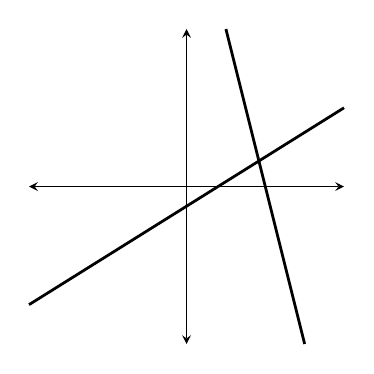
\begin{tikzpicture}[scale=.5]
             
              \draw[<->] (-4,0)--(4,0);
              \draw[<->] (0,-4)--(0,4);
             
             \draw[line width=1pt](-4, -3)--(4,2);
             \draw[line width=1pt](3, -4)--(1,4);
                 
            \end{tikzpicture}
            \end{center}
          \item Second, the two lines may have no points in common.  If this is the case, the system has no solutions.  We say that the system is \dfn{inconsistent}. 
          \begin{center}
            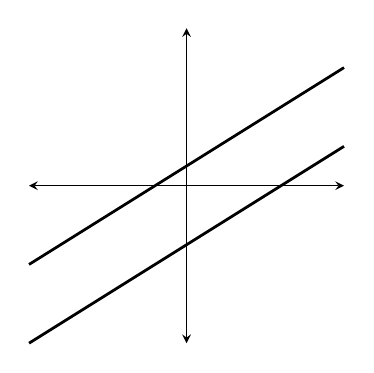
\begin{tikzpicture}[scale=.5]
             
              \draw[<->] (-4,0)--(4,0);
              \draw[<->] (0,-4)--(0,4);
             
             \draw[line width=1pt](-4, -4)--(4,1);
             \draw[line width=1pt](-4, -2)--(4,3);
                 
            \end{tikzpicture}
            \end{center}
          \item Finally, the two lines may coincide.  In this case, there are infinitely many points that satisfy both equations simultaneously.  We say that the system is consistent and has infinitely many solutions.
          \begin{center}
          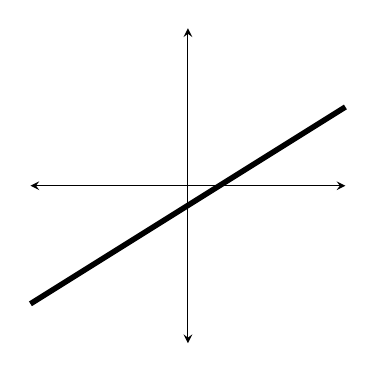
\begin{tikzpicture}[scale=.5]
           
            \draw[<->] (-4,0)--(4,0);
            \draw[<->] (0,-4)--(0,4);
           
           \draw[line width=2pt](-4, -3)--(4,2);
            
               
          \end{tikzpicture}
          \end{center}
          \end{itemize}
      
                  Given a linear system in two variables and more than two equations, we have a variety of geometric possibilities.  In terms of the number of solutions, there are three possibilities.
       
                  \begin{itemize}
                  \item First, it is possible for the graphs of all equations in the system to intersect at a single point, giving us a unique solution. 
                   
                  \begin{center}
                  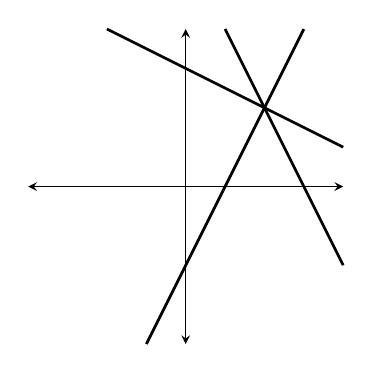
\begin{tikzpicture}[scale=.5]
                   
                    \draw[<->] (-4,0)--(4,0);
                    \draw[<->] (0,-4)--(0,4);
                   
                   \draw[line width=1pt](-2, 4)--(4,1);
                   \draw[line width=1pt](3, 4)--(-1,-4);
                   \draw[line width=1pt](1, 4)--(4,-2);
                       
                  \end{tikzpicture}
                  \end{center}
                   
                  \item Second, it is possible for the graphs to have no points common to all of them.  If this is the case, the system is inconsistent.
                   
                  %\begin{center}[3in]
                  \begin{center}
                  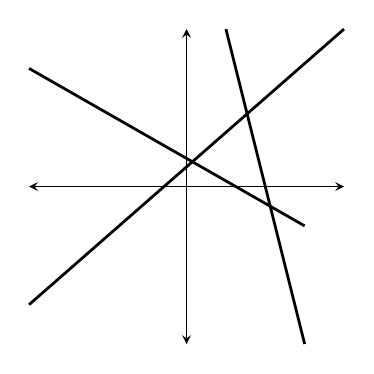
\begin{tikzpicture}[scale=.5]
                   
                    \draw[<->] (-4,0)--(4,0);
                    \draw[<->] (0,-4)--(0,4);
                   
                   \draw[line width=1pt](-4, -3)--(4,4);
                   \draw[line width=1pt](3, -4)--(1,4);
                   \draw[line width=1pt](3, -1)--(-4,3);
                       
                  \end{tikzpicture}\quad\quad
                  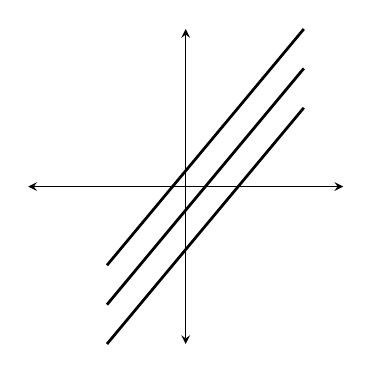
\begin{tikzpicture}[scale=.5]
                   
                    \draw[<->] (-4,0)--(4,0);
                    \draw[<->] (0,-4)--(0,4);
                   
                   \draw[line width=1pt](-2, -3)--(3,3);
                   \draw[line width=1pt](-2, -2)--(3,4);
                   \draw[line width=1pt](-2, -4)--(3,2);
                       
                  \end{tikzpicture}
                  \end{center}
                  %\end{center}
                   
                  \item Finally, it is possible for all of the lines to coincide, giving us infinitely many solutions.
                  \end{itemize}
  
    \end{exploration}
    
  \begin{exploration}\name{Geometry of Linear Systems in Three Variables}
    Let's now consider the following  system of three equations and three unknowns

    $$\begin{array}{ccccccc}
        3x & -&y&+&z&= &0 \\
        2x& +&y&+&2z&=&2\\
        x& +&4y&-&2z&=&11.
    \end{array}$$

    Introducing a third variable means that each equation describes a plane in $\mathbb{R}^3$, rather than a line in $\mathbb{R}^2$.  Luckily, we again preserve the solution set by the same row operations, so our strategy for solving systems of equations remains the same.

    \begin{example}

        Use the GeoGebra environment to solve the system of equations above. 

        \geogebra{stvqh3ts}{853}{364}

        \begin{hint}

            The solution to the system is $(1,2,-1)$, as depicted in the GeoGebra environment. If your constant terms are different, you may have made a mistake in your row operations.

        \end{hint}

        \begin{solution}

            The system can be solved by the following row operations (you may first need to swap rows to get the order to match the stated system above):

            %I NEED TO COME BACK AND JUST DO FRACTIONs

            $$R_2\rightarrow R_2-2R_3$$

            $$R_1\rightarrow R_1-3R_3$$

            $$R_2\rightarrow -R_2/7$$

            $$R_1\rightarrow R_1+13R_2$$

            $$R_3\rightarrow R_3-4R_2$$

            $$R_1\rightarrow -R_1/4.14$$

            $$R_2\rightarrow R_2+.86R_1$$

            $$R_3\rightarrow R_3-1.43R_1$$

            $$R_1\leftrightarrow R_3$$

            This gives the system 

            $$\begin{array}{ccccccc}
                 1x& +0y&+0z &=&1 \\
                0x&+1y& +0z& =&2\\
                0x &+1y &+1z 1z&=&-1.
            \end{array}$$

        \end{solution}
    \end{example}

    \begin{remark}

        Notice that the final system visualized as entirely horizontal or vertical planes, corresponding to the equations $x=1$, $y=2$, and $z=-1$. This reduction to standard planes has an important corrolary in the next section, where we examine row operations from the perspective of matrices. 

    \end{remark}

    Now, let's use row operations to determine the geometry of less nice systems.

\begin{example}

    Use the GeoGebra environment to analyze the following system of equations, which again creates the third equation from the first two via linear combination:

    $$\begin{array}{ccccccc}
        2x & +&3y&-&z&= &5 \\
        x& -&y&+&4z&=&6\\
        4x& +&y&+&7z&=&17.
    \end{array}$$

    As always, use row operations to solve the system. We're going to pay particular attention to the format of the "solved" system at the end of this section, and in the coming sections as well.

    \begin{solution}

        While you don't need to know this to solve the system using row operations, the third row is created from $R_1+2*R_2$. So, again, the geometric reason that we don't have a solution is that the first two planes intersect at a line (rather than a point) and then the third plane doesn't change the solution set of the system, and hence does not create a new intersection point.

        Solving the system using row operations (without the knowledge above) can be done in steps simlar to the following:

        $$R_3\rightarrow R_3-4R_2$$

        $$R_1\rightarrow R_1-2R_2$$

        At this stage, note that $R_1$ and $R_3$ are the exact same equations, and so we can get rid of one by subtracting the other.

        $$R_1\rightarrow R_1-R_3$$

        Now, we see just the two "spanning" planes of the system, and can further reduce them as much as possible, but not likely to standard vertical or horizontal planes.

        $$R_3\rightarrow R_3/5$$

        $$R_2\rightarrow R_2+R_3$$

        $$R_1\rightleftarrows R_2$$

        $$R_2\rightleftarrows R_3$$

        This gives the system, in its most reduced form:

        $$\begin{array}{ccccccc}
            1x& +0y&+2.2z &=&4.6 \\
            0x&+1y& -1.8z& =&-1.4\\
            0x &+0y &+0z &=&0.
        \end{array}$$

        So, here, we again have infinitely many solutions, as any point along the intersecting line between the two planes will satisfy the system.

        In this case, let's set $z=\tau$, which is an unknown constant value. This changes the system to be 

        $$\begin{array}{ccccccc}
            1x& +0y&+2.2\tau &=&4.6 \\
            0x&+1y& -1.8\tau& =&-1.4\\
            0x &+0y &+0\tau &=&0.
        \end{array}$$

        Note that the third equations is still true for any number $\tau$. Then since $\tau$ is just some unknown constant, we can solve for $x$ and $y$, getting

        $$x=4.6-2.2\tau$$
        
        $$y=-1.4+1.8\tau.$$

        So any points of the form $(4.6-2.2\tau, -1.4+1.8\tau, \tau)$ will satisfy the system.

    \end{solution}

\end{example}

\end{exploration}

\begin{exploration}\name{Review: Possible Outcomes of 3x3 Systems}

We'll be unpacking more examples of systems with or without solutions in the homework, but here's an overview of the different ways that solutions can or can't exist for 3x3 systems of equations.

Given a linear system of three equations in three variables, there are three ways in which the system can be consistent.

\begin{itemize}
    \item First, the three planes could intersect at a single point, giving us a unique solution.
    \begin{center}
        \tdplotsetmaincoords{70}{130}
            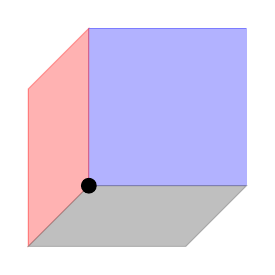
\begin{tikzpicture}
        \filldraw[blue, opacity=0.3](0,0,0)--(2,0,0)--(2,2,0)--(0,2,0)--cycle;
        \filldraw[red, opacity=0.3] (0,0,0)--(0,0,2)--(0,2,2)--(0,2,0)--cycle;
        \filldraw[gray, opacity=0.5] (0,0,0)--(0,0,2)--(2,0,2)--(2,0,0)--cycle;
        \fill[] (0,0,0) circle (0.1cm);
            \end{tikzpicture}
        \end{center}
    \item Second, the three planes can intersect in a line, forming a paddle-wheel shape.  In this case, every point along the line of intersection is a solution to the system, giving us infinitely many solutions.
        \begin{center}
        \tdplotsetmaincoords{70}{130}
                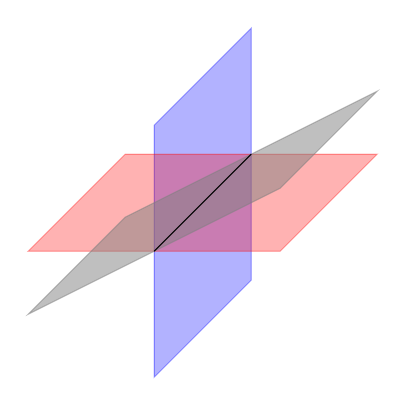
\begin{tikzpicture}[scale=0.8]
                \filldraw[blue, opacity=0.3](0,-2,2)--(0,2,2)--(0,2,-2)--(0,-2,-2)--cycle;
                \filldraw[red, opacity=0.3] (2,0,2)--(-2,0,2)--(-2,0,-2)--(2,0,-2)--cycle;
                \filldraw[gray, opacity=0.5] (2,1,2)--(2,1,-2)--(-2,-1,-2)--(-2,-1,2)--cycle;
                \draw[-](0,0,-2)--(0,0,2) ;
            \end{tikzpicture}
            \end{center}
    \item Finally, the three planes can coincide.  If this is the case, there are infinitely many solutions.
        \begin{center}
        \tdplotsetmaincoords{70}{130}
            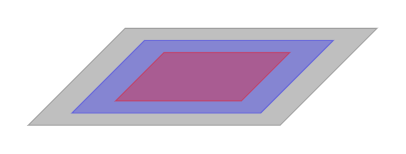
\begin{tikzpicture}[scale=0.8]
                \filldraw[gray, opacity=0.5] (2,0,2)--(-2,0,2)--(-2,0,-2)--(2,0,-2)--cycle;
                \filldraw[blue, opacity=0.3] (1.5,0,1.5)--(-1.5,0,1.5)--(-1.5,0,-1.5)--(1.5,0,-1.5)--cycle;
                \filldraw[red, opacity=0.3] (1,0,1)--(-1,0,1)--(-1,0,-1)--(1,0,-1)--cycle;
            \end{tikzpicture}
        \end{center}
\end{itemize}

There are four ways for a system to be inconsistent.  They are depicted below.
%\begin{center}[4in]
\begin{center}
\tdplotsetmaincoords{70}{130}
    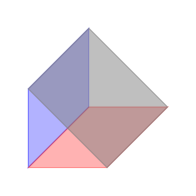
\begin{tikzpicture}[scale=0.5]
        \filldraw[blue, opacity=0.3](0,0,2)--(0,2,2)--(0,2,-2)--(0,0,-2)--cycle;
        \filldraw[red, opacity=0.3] (2,0,2)--(0,0,2)--(0,0,-2)--(2,0,-2)--cycle;
        \filldraw[gray, opacity=0.5] (0,2,2)--(0,2,-2)--(2,0,-2)--(2,0,2)--cycle;
    \end{tikzpicture}\quad
    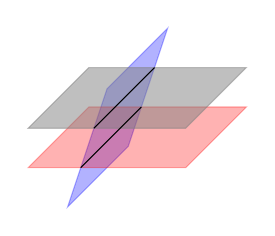
\begin{tikzpicture}[scale=0.5]
        \filldraw[blue, opacity=0.3](-1,-1,2)--(0,2,2)--(0,2,-2)--(-1,-1,-2)--cycle;
        \filldraw[red, opacity=0.3] (2,0,2)--(-2,0,2)--(-2,0,-2)--(2,0,-2)--cycle;
        \filldraw[gray, opacity=0.5] (2,1,2)--(-2,1,2)--(-2,1,-2)--(2,1,-2)--cycle;
        \draw[-](-2/3,0,-2)--(-2/3,0,2) ;
        \draw[-](-1/3,1,-2)--(-1/3,1,2) ;
    \end{tikzpicture}\quad
    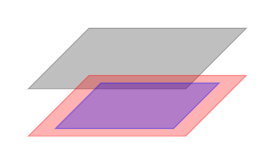
\begin{tikzpicture}[scale=0.5]
        \filldraw[gray, opacity=0.5] (2,1.2,2)--(-2,1.2,2)--(-2,1.2,-2)--(2,1.2,-2)--cycle;
        \filldraw[red, opacity=0.3] (2,0,2)--(-2,0,2)--(-2,0,-2)--(2,0,-2)--cycle;
        \filldraw[blue, opacity=0.3] (-1.5,0,1.5)--(-1.5,0,-1.5)--(1.5,0,-1.5)--(1.5,0,1.5)--cycle;
    \end{tikzpicture}\quad
    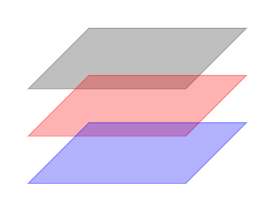
\begin{tikzpicture}[scale=0.5]
        \filldraw[gray, opacity=0.5] (2,1.2,2)--(-2,1.2,2)--(-2,1.2,-2)--(2,1.2,-2)--cycle;
        \filldraw[red, opacity=0.3] (2,0,2)--(-2,0,2)--(-2,0,-2)--(2,0,-2)--cycle;
        \filldraw[blue, opacity=0.3] (2,-1.2,2)--(-2,-1.2,2)--(-2,-1.2,-2)--(2,-1.2,-2)--cycle;
    \end{tikzpicture}
\end{center}

\end{exploration}

In the next chapter, we'll apply these ideas to the notion of matrix inverses, which take a much more intentional orientation towards interpreting these operations for matrices, and determining whether the matrix equation 

$$A\vec{x}=\vec{b}$$

can be solved by finding an inverse matrix $A^{-1}$ that satisfies

$$\vec{x}=A^{-1}A\vec{x}=A^{-1}\vec{b}$$


\end{document}